\documentclass[12pt,letterpaper]{article}
\usepackage{amsmath}
\usepackage{amsfonts}
%\usepackage{color}
\usepackage[usenames,dvipsnames]{color}
\usepackage{graphicx}
\usepackage{longtable}
\usepackage{rotating}
\usepackage{verbatim}
\usepackage[pdftex,bookmarksopen]{hyperref}
\hypersetup{pdfauthor={John Sibert}}
\hypersetup{pdfsubject={Compartment model of MHI YFT}}
\hypersetup{pdftitle={Two-compartment models of Main Hawaiian Islands
Yellowfin Tuna Population}}
\hypersetup{pdfkeywords={yellowfin,state space,compartment model,Hawaii}}

\newcommand\doublespacing{\baselineskip=1.6\normalbaselineskip}
\newcommand\singlespacing{\baselineskip=1.0\normalbaselineskip}
\renewcommand\deg[1]{$^\circ$#1}
\newcommand\SD{SEAPODYM}
\newcommand\MFCL{MULTIFAN-CL}
\newcommand\ADMB{ADModel Builder}
\newcommand\SPC{Secretariat of the Pacific Community}
\newcommand\WCPO{Western Central Pacific Ocean}
\newcommand\SSAP{Skipjack Survey and Assessment Programme}
\newcommand\RTTP{Regional Tuna Tagging Programme}
\newcommand\PTTP{Pacific Tuna Tagging Programme}
\newcommand\FAD{fish aggregating device}
\newcommand\ADRM{advection-diffusion-reaction model}
\newcommand\help[1]{\color{Magenta}{\it #1 }\normalcolor}
\newcommand\widebar[1]{\overline{#1}}
\newcommand\EEZ{Exclusive Economic Zone}

\newcommand\None{{N_{1,1}}}
\newcommand\Ntwo{{N_{2,1}}}
\newcommand\Nsum{{N_{1,1}+N_{2,1}}}
\newcommand\peryr{yr$^{-1}$}
\newcommand\prevN[1]{{#1_{t-\Delta t}}}
\newcommand\nextN[1]{{#1_t}}

\title{Two-compartment models of Main Hawaiian Islands Yellowfin Tuna
Population\\
Interim Report}

\author{
John Sibert\thanks{sibert@hawaii.edu}\\
Joint Institute of Marine and Atmospheric Research\\
University of Hawai'i at Manoa\\
Honolulu, HI  96822 U.S.A.\\[0.125in]
\date{\today}
}

\pagestyle{myheadings}
\markright{Sibert\hfil MHI Comparment Model\hfil{\bf DRAFT}\hfil\today}

\begin{document}
\maketitle

\doublespacing

\section*{Introduction}
The Yellowfin Tuna (YFT) population in main Hawaiian Islands (MHI) is
embedded in a larger pan-Pacific stock. Nevertheless, local fishermen
believe that the MHI supports a ``resident'' yellowfin population.
Some scientific observations are consistent with this belief. 
Recent tagging, tracking and
studies show that the rate of exchange between the MHI population
and the larger stock is low (Itano and Holland 2000). Analysis
of YFT otoliths sampled from
throughout the Pacific conclude that approximately 90\% of the MHI
population was reared in the MHI (Wells et al 2012).
The Hawaii based longline along with various small-scale fisheries
land a combined catch
approximately 5000 mt of YFT annually (ref). Management of these
fisheries is an important an important  local issue deserving of scientific support.

This paper explores some potential models that might be used to
analyze options for the management of fisheries for YFT in the MHI.

The principle assumptions for modeling the MHI YFT population are:
\begin{enumerate}
\item The Pacific Ocean near Hawaii is divided into two regions:
MHI (region 1) and elsewhere (region 2); see Figure~\ref{fig:MHImap}.
\item Fish emigrate from region 1 to region 2, but emigrant fish have
no effect on region 2 population dynamics. Region 2 is an ``infinite
sink''.
\item Fish immigrate from region 2 to region 1, and mix completely.
\item Immigrant fish are indistinguishable from ``resident'' fish
(i.e. both groups of fish have the same population dynamics) and
interact with the fishing gear identically.
\item Immigration into the MHI is dependent on the
biomass of the yellowfin population outside of the MHI as estimated by
some other model, e.g., \MFCL\ or \SD.
\item The fishery comprises of several gear types, each with characteristic
fishing mortality.
\item The evolution of fishing mortality over time is a random walk
where the current fishing mortality in the current time step is equal
to the fishing mortality in the previous time step plus a random deviation
(equation~\ref{eqn:Fwalk}).
\end{enumerate}

\section*{Data}
Several sources of data used are used in this analysis:
\begin{enumerate}
\item  Yellowfin catch weights reported to the Hawaii Department of Aquatic
Resources (HDAR) from 1949 to 2014 from the  Offshore Handline, Toll,
Inshore Handline, Longline, and Aku Boat fleets.
\item Longline yellowfin catch weights reported to the National Oceanic and
Atmospheric Administration, National Marine Fisheries Service (NOAA)
under the federally mandated log book program from 1995 through 2013.
\item Measurements of individual yellowfin weights fish sampled at the
Honolulu auction by NMFS staff from 2000 through 2013.
\item Model estimates of yellowfin biomass for MFCL regions 2 and 4
provided by the Oceanic Fisheries Programme at the Secretariat of the
Pacific Community (SPC) in Noumea, New Caledonia. These estimates span
the period 1952 through 2012.
\end{enumerate}
All data are reported by quarter of the year.

%The Hawaii longline fishery has a long history and changed radically
%in the 1990s when new vessels entered the fleet and fishing gear was
%modernized.
%The HDAR longline data covers the period 1949 through 2001 and does
%not differentiate between ``deep'' and ``shallow'' sets.
%The NOAA longline data covers the period 1995 through 2013 and reports deep
%and shallow set set separately.
%Thus the period of most radical change is included in time series.

%[1] Aku boat          Bottom/inshore HL Longline          Other            
%[5] Troll             Tuna HL           Casting           Hybrid           
%[9] Shortline         Vertical line    

% statistics of catch time series first differences
%TS                 Mean     S. D.
%OffshoreHL  0.017659002 0.5994987
%Troll       0.018124404 0.7051216
%Longline    0.002425213 0.7782023
%InshoreHL  -0.002342312 0.6935796
%AkuBoat    -0.004970204 1.0908600



The HDAR data comprise catch reports for the following gear
categories"
``Aku boat'',``Bottom/inshore HL'',``Longline'',
``Troll'',``Tuna HL'',``Casting'',``Hybrid'',
``Shortline'',``Other'',and ``Vertical line''.
For this analysis catches by ``Casting'',``Hybrid'',
``Shortline'',``Other'',and ``Vertical line'' are combined into a new
category, ``Misc.''. The ``Misc'' catches are highest after year 2000,
but represent a small proportion of the catch.
The catch time series for the HDAR data are shown in
Figure~\ref{fig:hdarTS}. These time
series exhibit marked quarterly cycles suggesting a strong seasonal
signal in the catches by all fleets.
Some series also contain sustained periods of zero catch which
document the development and subsequent shift away from a specific
gear type. It is assumed that these declines in catches represent a
``collapse'' of a fishery due more to social and economic factors than
to a decline of stock.
Some time series are punctuated by brief, on or two quarters in
length, of zero catches. Again it is assumed that these zero catches
are not caused by low stock levels.
The ``Aku Boat'' fishery was a small pole and line fishery
targeting skipjack tuna in Hawaii, for which yellowfin was an
incidental catch ceased operation because of
problems marketing fresh skipjack.

The longline fishery has changed drastically over time. In the late
1940s, it was a relatively small fishery using traditional
Okinwawan-style gear \help{(reference)}, usually labeled ``flag
line''. Participation in this fishery generally declined from 1950 to
late 1980s, as can be seen in the time series plots. In the 1990s, the longline
fishery expanded rapidly with the introduction of US fishing boats
from the Atlantic ocean with modern monofilament longline gear and
deeper sets.

Figure~\ref{fig:hdarTS} also displays the first order differences
between successive quarters. This statistic emphasizes the seasonal
periodicity of all fishing fleets and helps to identify potential anomalies in
the data such as changes in reporting protocol. Some possible
anomalies can be seen in the late 1980s in the Tuna HL fleet, the
early 1990s in the longline fleet, and the mid 1950s in the Aku Boat
fleet. 

The partial autocorrelations within each time
series are shown in Figure~\ref{fig:catchPACF}. These correlations
confirm the periodic nature of the catch time series which have
significant positive correlations at lags of 1,3 and 4 quarters.


NOAA began to collect data from the longline fleet under a federally
mandated logbook program in 1990, and in 1995 the deep and shallow
setting are distinguished in the data. The HDAR data does not
distinguish between deep and shallow sets.
Figure~\ref{fig:hdarnoaaLLTS} shows the correspondence between the
HDAR and NOAA time series. The combined deep plus shallow catches from
NOAA line up fairly well with the overlaping HDAR data. The simple
average of the HDAR data with the combined NOAA deep plus shallow data
appears to have iroughtly the same autocorrelation structure as the
constituent time series, Figure~\ref{fig:LLpartialacf}.
\help{Data are also available from NOAA for the period 1990-1995, but
have not yet been included in this analysis.}


\begin{figure}
\begin{center}
\includegraphics[height=0.9\textheight]{./graphics/hdar_catch_history.png}
\caption{\label{fig:hdarTS}
Yellowfin catch in metric tonnes by principle fisheries operating in
the Main Hawaiian Islands from the HDAR data.
The dotted red line superimposed on each time series is the difference in
catch between successive quarters.
The red tick marks on the abscissa indicate quarters where catches
were zero.
}
\end{center}
\end{figure}

\begin{figure}
\begin{center}
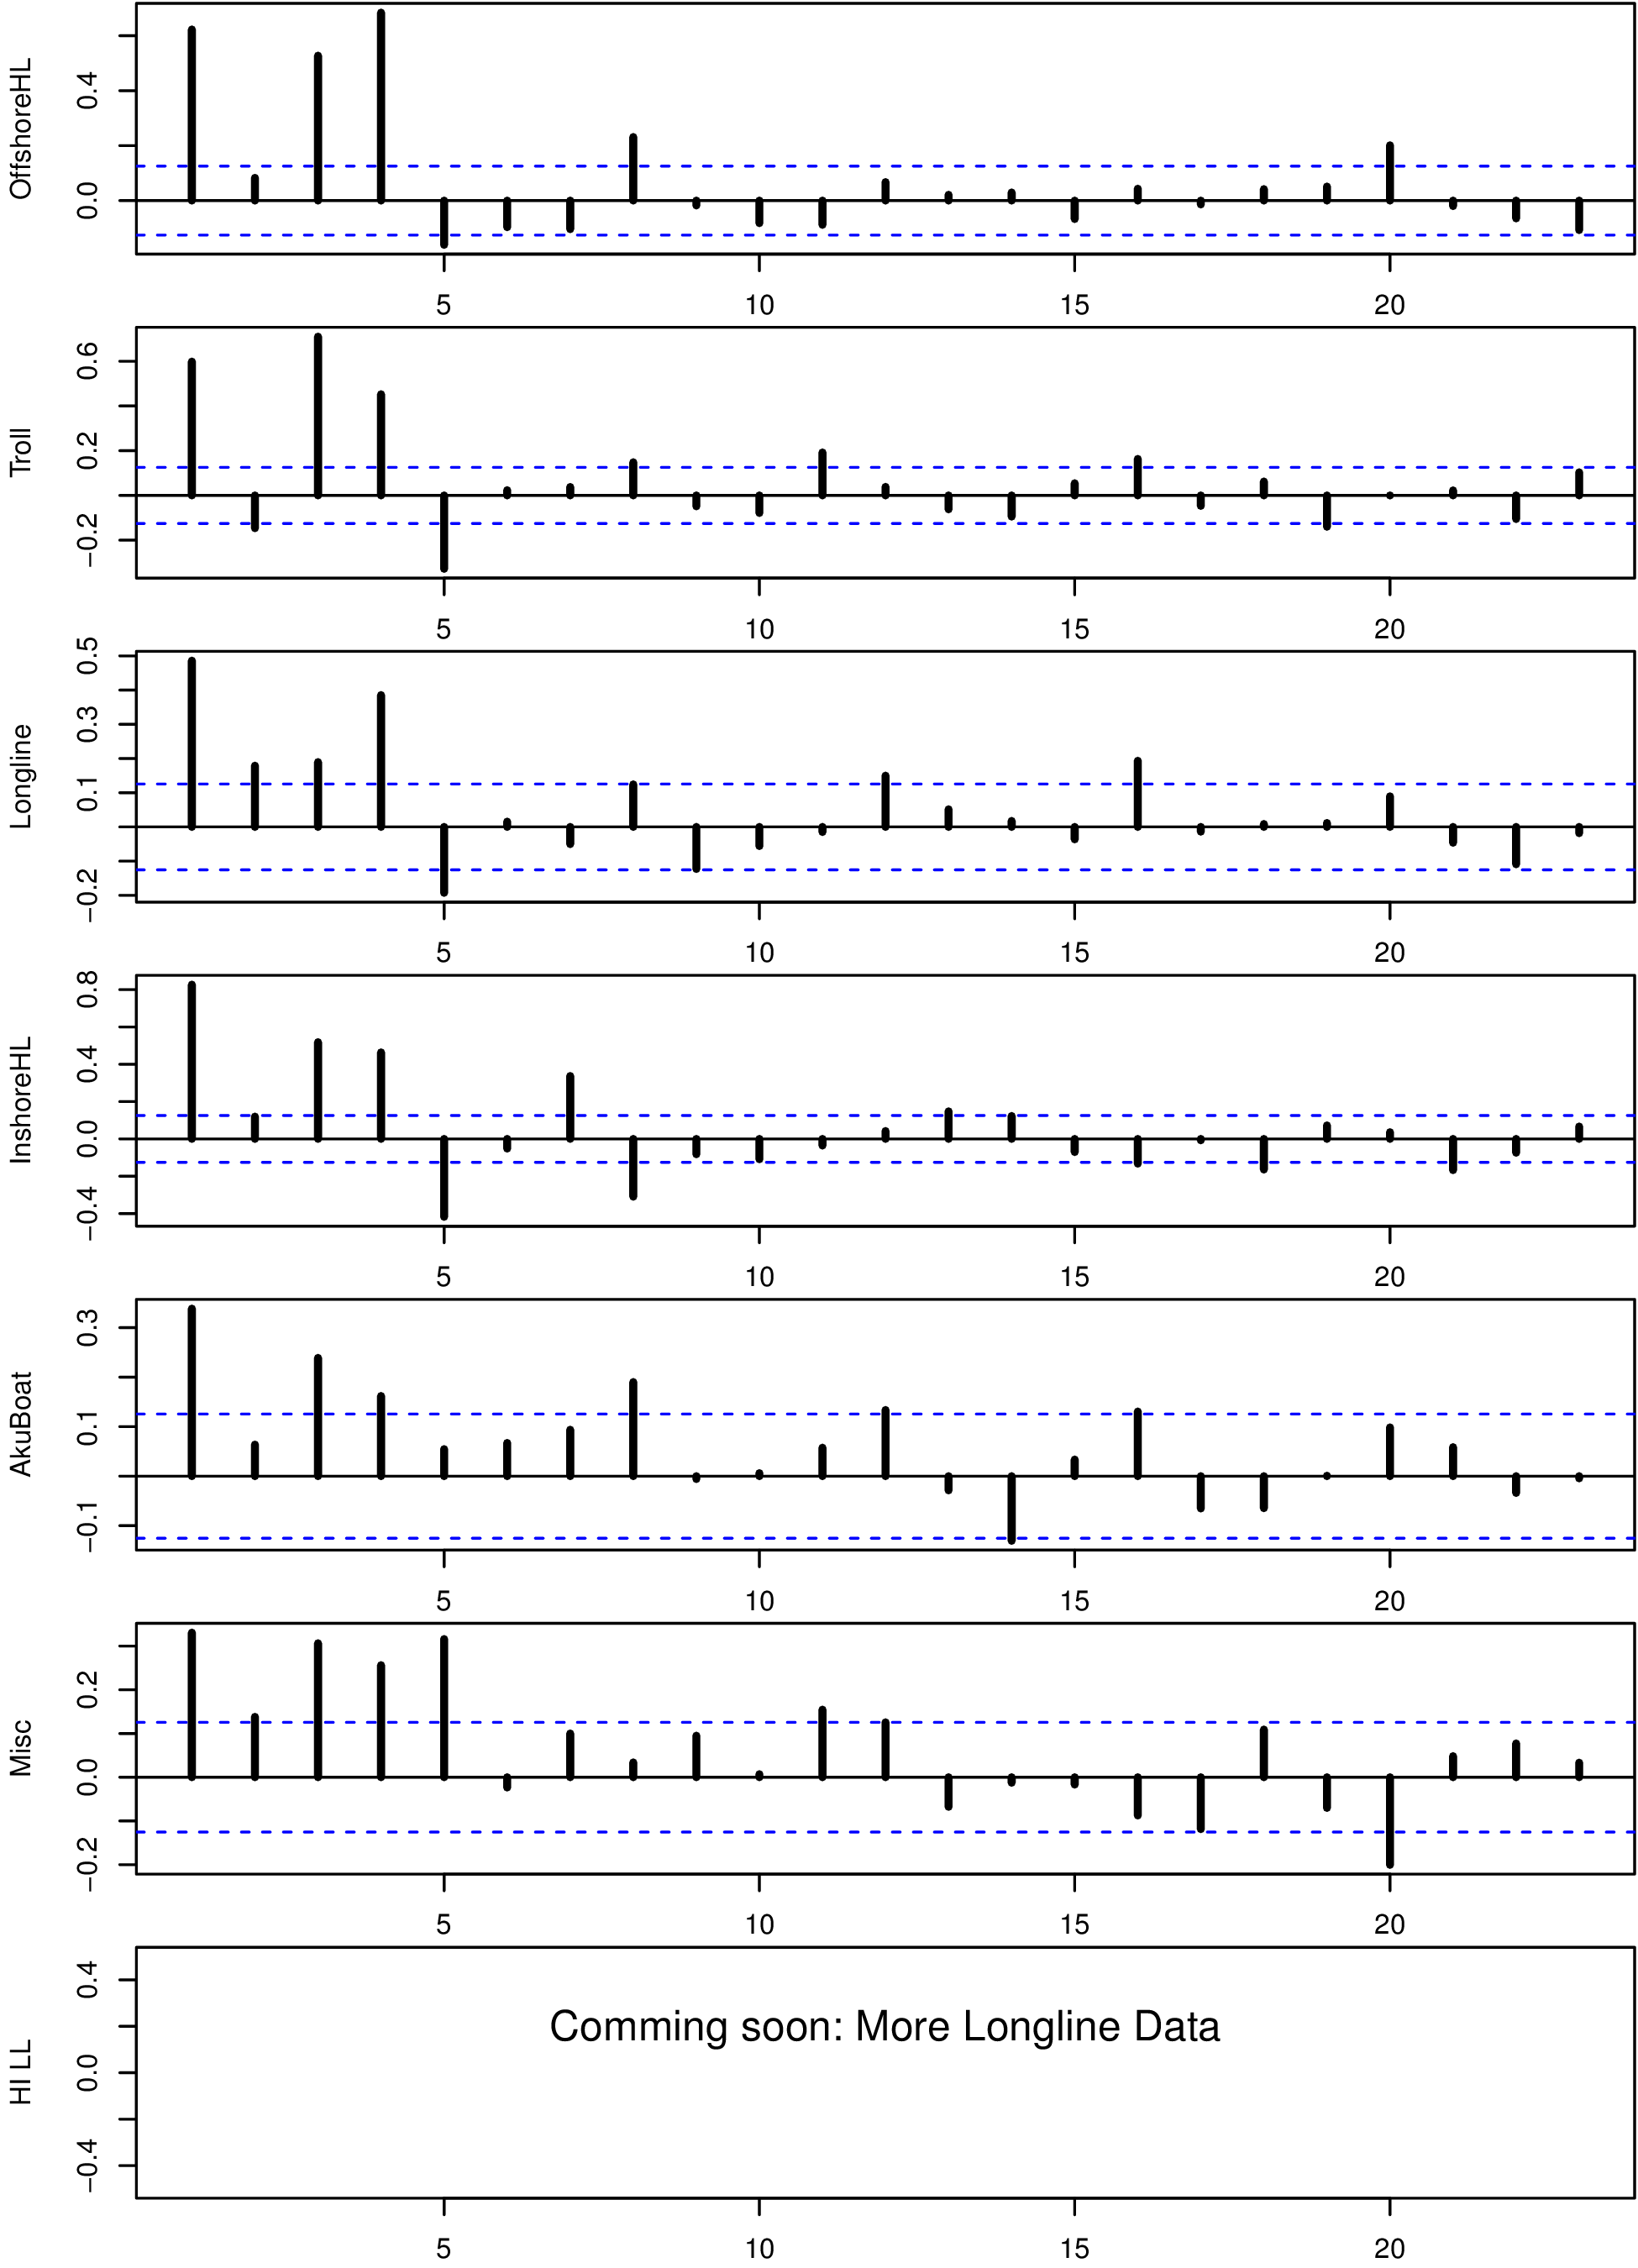
\includegraphics[height=0.9\textheight]{./graphics/partial_acf.png}
\caption{\label{fig:catchPACF}
Partial autocorrelation coefficients of the catch time series. The
dashed blue lines indicate approximate 95\% confidence limits of the
correlations.}
\end{center}
\end{figure}

\begin{figure}
\begin{center}
\includegraphics[height=0.9\textheight]{./graphics/hdar_noaa_LL_ts.png}
\caption{\label{fig:hdarnoaaLLTS}
Comparison between HDAR and NOAA longline time series. The upper panel
shows the NOAA deep and shallow set data superimposed on the HDAR
data. The lower panel shows the time series produced by a simple
average of the HDAR data and the sum of the NOAA deep and shallow
catches.}
\end{center}
\end{figure}

\begin{figure}
\begin{center}
\includegraphics[height=0.9\textheight]{./graphics/LL_partial_acf.png}
\caption{\label{fig:LLpartialacf}
Partial autocorrelations within the NOAA and combined time
series. F refers to the HDAR longline data, D refers to the NOAA deep
set data, S to the shallow set data,
DS to the combined deep and shallow set data, and Mean to the average
of the HDAR and NOAA deep plus shallow.
}
\end{center}
\end{figure}

%\begin{figure}
%\begin{center}
%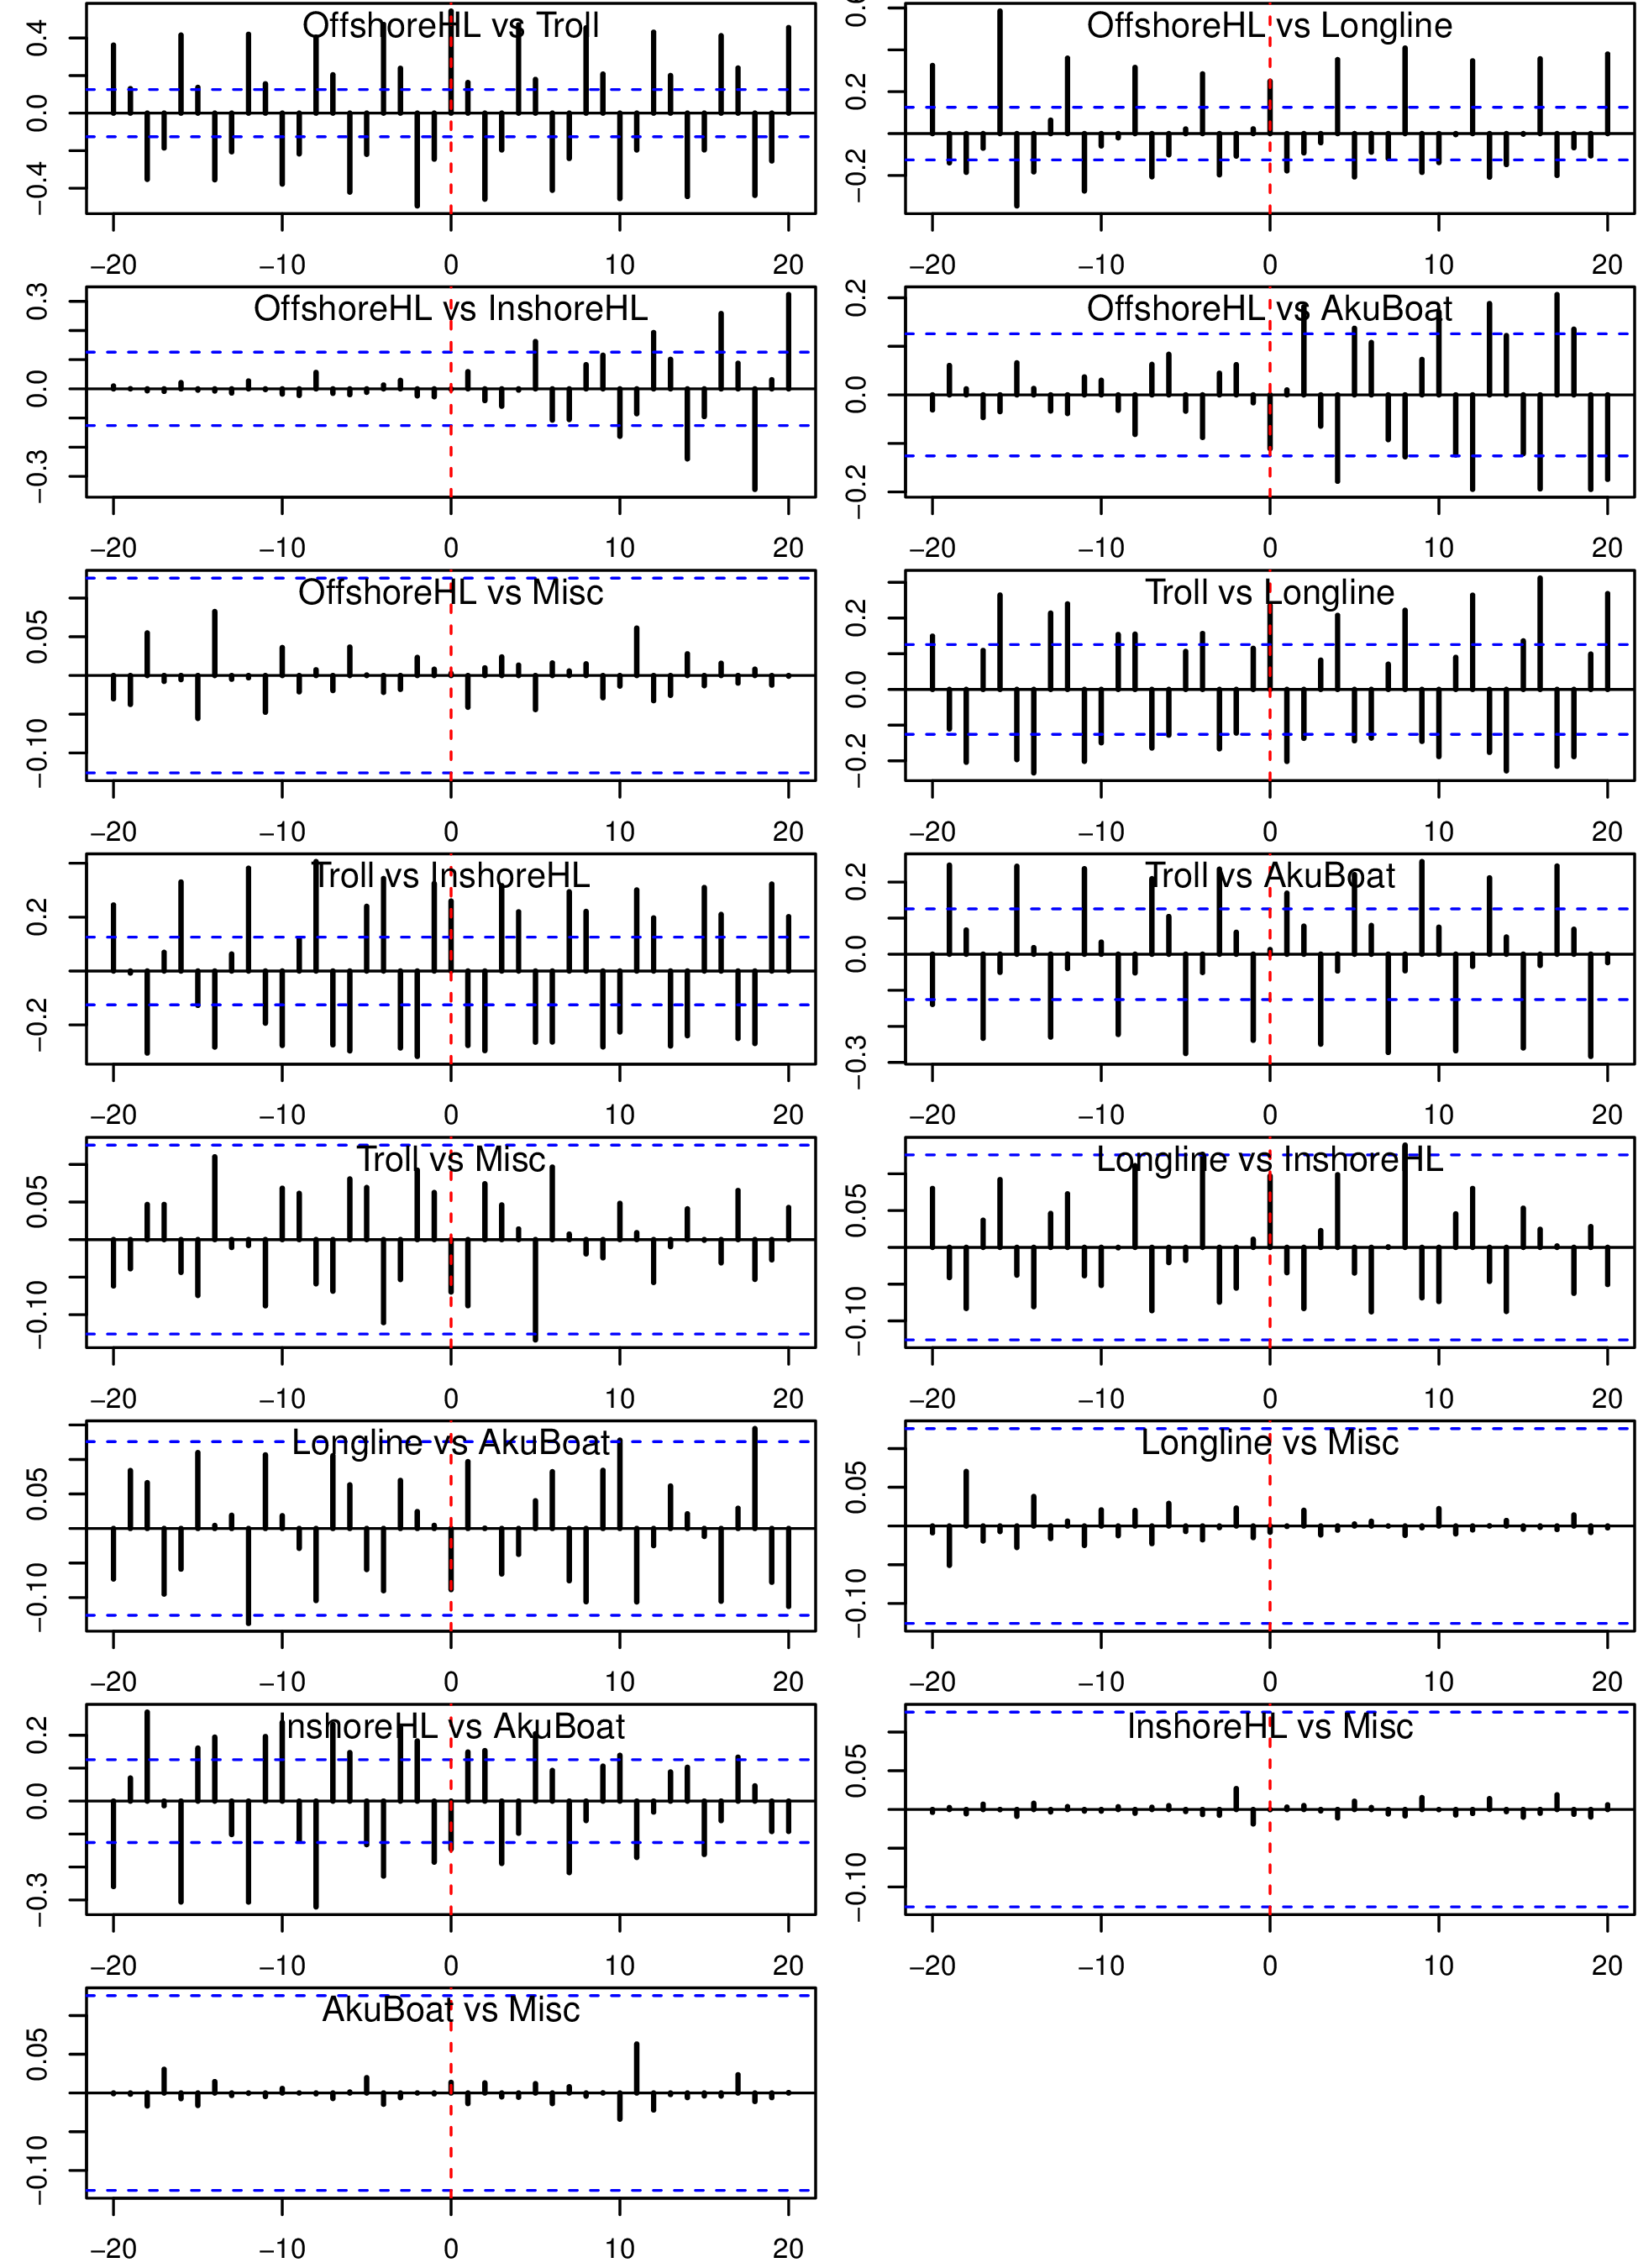
\includegraphics[height=0.9\textheight]{./graphics/ccf.png}
%\caption{\label{fig:catchCCF}
%Cross correlation coefficients between pairs of the first order
%differences of each catch time series at different lags.
%The vertical dashed red line emphasize zero lag.
%The dashed blue lines indicate approximate 95\% confidence limits of
%the correlation coefficients.}
%\end{center}
%\end{figure}

\clearpage
\section*{Models}
The general modeling approach to be applied will be similar to the
state-space model utilized by Nielsen and Berg (2014). 
State-space models separate variability in the biological
processes in the system (transition model)
from errors in observing features of interest
in the system (observation model). 
The general form of the transition equation is
\begin{equation}
\alpha_t=T(\alpha_{t-1}) + \eta_t
\end{equation}
where the function $T$ embodies the stock dynamics, describing the
development of the state at time $t$ from the state at the previous
time with random process error, $\eta$.
Similarly the general observation equation is
\begin{equation}
x_t = O(\alpha_t) + \varepsilon_t
\end{equation}
where the function $O$ describes the measurement process and with
error $\varepsilon$
Separation if process from measurement offers statistical advantages in
estimating model parameters.

Fishing effort is not observed and fishing mortality is
modeled explicitly. The logarithm of fishing mortality is assumed to
follow a random walk with normal increments, i.e.
\begin{equation}
\log F_{g,t} = \log F_{g,t-1} + \xi_{g,t},\qquad {\rm where}\;
\xi_{t,g}\sim N(0,\sigma_g)
\label{eqn:Fwalk}
\end{equation}
where  $\sigma^2_g$ is the characteristic variance of the fishing
effort random walk for fleet $g$.

\subsection*{Age-aggregated model: logistic population dynamics (Schaefer Model)}

Let $\None$ equal the population size of fish originating in region 1
and residing in region 1
and $\Ntwo$ equal the population size of fish originating in region 2
but residing in region 1.
The total population size of fish residing in region 1 is thus
$\Nsum$, and the dynamics of the population in region 1 is represented as
\begin{equation}
\frac{d}{dt}\big(\Nsum\big)=\big(\Nsum\big)\Big[r\Big(1-\frac{\Nsum}{K}\Big)-F-T_{12}\Big]+T_{21}
\label{eqn:logistic}
\end{equation}
where $r$ is the per capita logistic growth rate per year $K$ is the
logistic ``carrying capacity'' measured in the same units as $\None$
and $\Ntwo$, $F$ is the total fishing mortality in region 1, and $T_{12}$
is the emigration rate from region 1 to region 2. $T_{21}$
is the annual rate of immigration of fish from region 2 to region 1
measured in the same units as $K$ per year.

Equivalent differential equations could be devised for the dynamics of
fish residing in region 2 (i.e., $\frac{dN_{2,2}}{dt}$ and
$\frac{dN_{1,2}}{dt}$) but 
the dynamics of the fish population in region 2 is external to this
model. $T_{21}$ can be considered to be form of population forcing
from the larger stock in which the MHI population is embedded, perhaps
estimated from other models, such as \MFCL\ or \SD, or perhaps
represented by an
autocorrelated stochastic process. The appearance of
$\Nsum$ in the numerator of the logistic term reflects the assumption
that the population dynamics fish immigrating into region 1 depend on
the population dynamics in region 1. This assumption leads to an
important non-linearity in the model that allows the possibility of
overwhelming of the
local stock by a more numerous immigrant stock as is often characteristics of
mixed-stock fisheries.

The ratio $\frac{\None}{\Nsum}$ is of potential interest, so
equation~\ref{eqn:logistic} needs to be expanded and rearranged
leading to a set of simultaneous differential equation for the
components of the population inhabiting region 1.
\begin{eqnarray}
\frac{d\None}{dt}&=&\None\Big[r\Big(1-\frac{\None}{K}\Big)
-F - T_{12}\Big] - \frac{r}{K}T_{12}\None\Ntwo\nonumber\\
\frac{d\Ntwo}{dt}&=&\Ntwo\Big[r\Big(1-\frac{\Ntwo}{K}\Big)
-F - T_{12}\Big] - \frac{r}{K}T_{12}\None\Ntwo + T_{21}
\label{eqn:coupledschaefer}
\end{eqnarray}
The non-linear term from equation~\ref{eqn:logistic} appears the term
$r\frac{\None\Ntwo}{K}$ in both of the above equations.

The equilibrium of this system can be found by setting
$\frac{d\None}{dt} = 0 = \frac{d\Ntwo}{dt}$. After some simplification
the result is $\frac{T_{21}}{\Ntwo} = 0$. In other words, there is no
equilibrium in this coupled system, other than the degenerate case of
no immigration ($T_{21}=0$) into the region 1. Thus, the notion of using
equilibrium-based reference points such as MSY to manage fisheries for
MHI yellowfin is ill advised.


The log transformed equivalent of equation~\ref{eqn:coupledschaefer} can be written as
\begin{eqnarray}
\frac{d\log(\None)}{dt}&=&r\Big(1-\frac{\None}{K}\Big) -F - T_{12} - \frac{r}{K}T_{12}\Ntwo\nonumber\\
\frac{d\log(\Ntwo)}{dt}&=&r\Big(1-\frac{\Ntwo}{K}\Big) -F - T_{12} - \frac{r}{K}T_{12}\None + T_{21}/\Ntwo
\label{eqn:coupledlogschaefer}
\end{eqnarray}

Equations \ref{eqn:coupledlogschaefer} are solved by finite difference
approximations using explicit time stepping.
\begin{eqnarray}
\log \None_t &=& \log \None_{t-\Delta t} +\Delta t\bigg(r\Big(1-\frac{\None_{t-\Delta t}}{K}\Big)
-F_{t-\Delta t} - T_{12} - \frac{r}{K}T_{12}\Ntwo_{t-\Delta t}\bigg)+\eta_{1,t}\nonumber\\
\log \Ntwo_t &=& \log \Ntwo_{t-\Delta t} +\Delta t\bigg(r\Big(1-\frac{\Ntwo_{t-\Delta t}}{K}\Big)
-F_{t-\Delta t} - T_{12} - \frac{r}{K}T_{12}\None_{t-\Delta t}\nonumber\\
     &+&T_{21}/\Ntwo_{t-\Delta t}\bigg)+\eta_{2,t}
\label{eqn:finitecoupledlogschaefer}
\end{eqnarray}
Addition of process error terms $\eta_{1,t}$ and $\eta_{2,t}$ yields a form suitable
for use as the transition equation in a state-space model.

The predicted catch in region 1 is the product of fishing mortality
and the total population in region, $\None+\Ntwo$.
Thus the observation model predicting catch in the region 1
under this model is
\begin{equation}
C_{g,t} = F_{g,t}\cdot(\None_{t-\Delta t}+\None_t+\Ntwo_{t-\Delta t}+\Ntwo_t)/2
\label{eqn:catcheqn}
\end{equation}
where the total population in region 1 is the sum of the average
population over the time step (Quinn and Deriso, 1999).

\vspace{4ex}
\noindent {\bf Acknowledgements.}
This work was funded by the Western Pacficic Regional Fisheries
Managment Council. I thank the Council for its generous support and
Council Staff Paul Dalzell and Eric Kingma for encouraging me to
actually take on this challenging project and for their on-going
collaboration.
Thanks to Mr. Reginald Kokubun of the Hawaii Division of Aquatic
Resources for supplying catch report data from the HDAR commercial
fisheries data base.
Thanks to Mr. Keith Bigelow and Ms. Karen Sender of NOAA Pacific
Island Fisheries Science Center for supplying logbook reporting data and
weight-frequency data from the PIFSC data base.
Thanks also to Dr. John Hampton of the Secretariat of the Pacific
Community, Oceanic Fisheries Programme, for making available
MULTICAN-CL output files from the latest Western and Central Pacific
Fisheries Commission yellowfin tuna stock assessment, and to Mr. Nick
Davies for sharing R scripts and advice to decode the MFCL output files.

\section*{References}
{\parindent=0cm \small
\everypar={\hangindent=2em \hangafter=1}\par
\doublespacing
Adam, M. S., J. Sibert, D. Itano and K. Holland. 2003. Dynamics of
bigeye (Thunnus obesus) and yellowfin tuna (T. albacares) in Hawaii's
pelagic fishery: analysis of tagging data with a bulk transfer model
incorporating size specific attrition. Fishery Bulletin 101(2):
215-228.

Davies, N., S. Harley, J. Hampton, S. McKechnie. 2014. Stock
assessment of yellowfin tuna in the western and central pacific ocean.
WCPFC-SC10-2014/SA-WP-04.

Itano, D., K. Holland. 2000.  Movement and vulnerability of bigeye
(Thunnus obesus) and yellowfin tuna (Thunnus albacares) in relation to
FADs and natural aggregation points.Aquat. Living Resour. 13: 213-223.

Kleiber, P., J. Hampton, N. Davies, S. Hoyle, D. Fournier. 2014.
MULTIFAN-CL User’s Guide

Nielsen, A. and C. Berg. 2014. Estimation of time-varying selectivity
in stock assessments usingstate-space models. Fisheries Research
158:96-101.

Quinn, T and R. Deriso. 1999. Quantitative fish dynamics. Oxford
University Press, New York.

Wells, D., J. Rooker, D. Itano. 2012.  Nursery origin of yellowfin
tuna in the Hawaiian Islands. Mar. Ecol. Prog. Ser. 461:187-196. 
\par}

%%%%%%%% figures begin here %%%%%%%%%%%%%%%%%%%%%%
\end{document}
